 \documentclass[11pt,a4paper]{article}
\usepackage[utf8]{inputenc}
\usepackage[finnish]{babel}
\usepackage[T1]{fontenc}
\usepackage{amsmath}
\usepackage{amsfonts}
\usepackage{amssymb}
\usepackage{amsthm}
\usepackage{url}
\pagestyle{plain}
\usepackage{graphicx}
\title{Eugenoli}
\author{Delun Li\\014631300\\Orgaanisen kemian työt 1\\Työ 3}
\date{20.10.2018}
\begin{document}

\maketitle

\pagebreak


\section{Johdanto}

Tässä työssä valmistettiin eugenolia neilikasta ja oppia höyrytislauksen käytäntöä.

\vspace{0.3cm}

\noindent Eugenolin rakennekaava:

\hspace{2.5cm}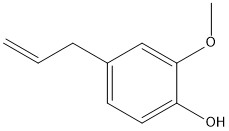
\includegraphics[]{eugenoli.jpg}

\vspace{0.3cm}

\noindent Höyrytislaus on eräänlainen tislausmenetelmä, jonka avulla saadaan tislattua ja puhdistettua lämpötilaherkille aineille. Aineiden höyrypaine ei laske, jos yhdisteessä on kaksi liukenematonta ainetta. Tällöin systeemin kokonaispaine on Daltonin osapainelain mukaan aineiden höyrypaineiden summa. 
Kun systeemin kokonaispaine saavuutta ulkoisen paineen kuumennettaessa, seos alkaa kiehua ja aineet tislautuvat. Tämän menetelmän avulla voidaan tislata orgaanisia yhdisteitä, jotka ovat veteen liukenettomia, pienemmässä lämpötilassa, missä yhdiste ei ehdi hajoamaan. $^1$

\section{Työn suoritus}

Seosta, jossa oli neilikkaa (10 g, 0,0609 mol) ja vettä (100 ml), tislattiin vesihöyrytislauslaitteistolla. Tämän jälkeen tislettä uutettiin CH$_2$Cl$_2$ (2x25 ml). Eristetty orgaaninen kerros uutettiin 5$\%$NaOH:illa (3x20 ml). Yhdistetyt vesikerrokset pestiin kerran CH$_2$Cl$_2$ (15 ml), jonka jälkeen hapetettiin happamaksi 2M HCl:lla ja uutettiin CH$_2$Cl$_2$ (2x25 ml). Yhdistetty orgaaninen kerros pestiin vedellä (10 ml) ja kuivatettiin Na$_2$SO$_4$:lla. Näiden jälkeen kirjattiin saanto (0,853 g, 8,5$\%$) ja ajettiin IR-spektri ja kaasugromatogrammi.

\section{Johtopäätökset}

Liitteessä \textbf{IR-spektri}:ssä on ajettu IR-spektri tuotteesta. 3200-3500 cm$^{-1}$ välillä näkyy eugenolin -OH ryhmän aiheuttamaa venytysvärähtelyä ja 3610 cm$^{-1}$ kuvaa hydroksyyliryhmän kiinittymistä aromaattiseen renkaaseen. Eetterin läsnäolon takia aaltoluvujen 1230-1310 välillä näkyy eetteriryhmän absorbointia. Aromaattisen renkaan olennaisia absrobointeja kuvaavat aaltoluvuilla 3030, 1450-1600, 560-900 ja 800-860. 1450-1600 kuvaa aromaattisen reankaan C$=$C värähtelyä, 860-900 kuvaa renkaassa olevaa eristynyttä vetyä ja 800-860 kuvaa renkaassa kahden vierekkäisten vetyjen olemassaolosta. Propeeni osa yhdisteestä kuvaavat 3080 cm$^{-1}$ ja 2925 cm$^{-1}$, missä 3080 kuvaa sp$^2$ $=$CH$_2$ sidoksen värähtelyä ja 2925 sp$^3$ -CH$_2$- värähtelyä.$^2$

Kun verrataan liitteitä \textbf{Kromatogrammi: Eugenoli}:a ja \textbf{Kromatogrammi: Kaupallinen eugenoli}:a, huomaataan molemmat olevan lähes samanlaisia. Molemmat piikit sijoittuvat 10 minuutin kohdalla. Tämän lisäksi tuotteen kromatogrammista ei löydy mitään muita olennaisia piikkejä. Liitteessä \textbf{Kromatogrammi: Etyyliasetaatti} on esitetty käytetyn liuottimen puhtautta ja kromatogrammia.

IR-spekrin ja kromatogrammien avulla voidaan sanoa, että saatu tuotteemme on eugenoli.  Saanto on toisaalta hyvin mitätöntä, sillä tislettä otettiin vain 200 ml talteen. Työ sujui ongelmitta, mutta pitää olla tarkka uutoissa ja uutoksen aikana uuttosuppiloon aiheutunutta yliapainetta.

\section{Viitteet}

1. \url{https://en.wikipedia.org/wiki/Steam_distillation}

\noindent 2. Tapio Hase, \textit{Tables for Organic Chemistry}, s. 20, 21, 22, 25, 26, 

\section{Liitteet}

IR-spektri

\noindent Kromatogrammi: Kaupallinen eugenoli 

\noindent Kromatogrammi: Eugenoli 

\noindent Kromatogrammi: Etyyliasetaatti

\end{document}
